\begin{figure}[h]
	\centering
	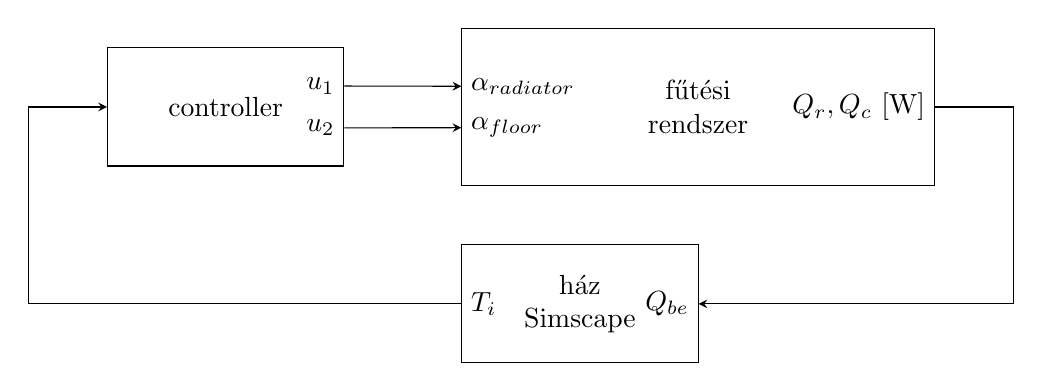
\begin{tikzpicture}[>=stealth]

	
	\node[draw,rectangle, minimum height=2cm,minimum width=6cm] (Heat) at (6,2.5) {\parbox{2cm}{\centering fűtési rendszer}};
	%\node[draw,rectangle, minimum height=2cm,minimum width=5.5cm] (Simsc) at (9,2.5) {\parbox{2cm}{\centering fűtési rendszer Simscape}};
	\node[draw,rectangle, minimum height=1.5cm,minimum width=3cm] (House) at (4.5,0) {\parbox{2cm}{\centering ház Simscape}};
	\node[draw,rectangle, minimum height=1.5cm,minimum width=3cm] (Control) at (0,2.5) {controller};
	
	\draw[->] (Control.350) node[left]{${u_{2}}$} --  (Heat.185) node[right]{$\alpha_{floor}$};  %node[above left]{$\alpha_{radiator}$}; 
	\draw[->] (Control.10) node[left]{${u_{1}}$} --  (Heat.175) node[right]{$\alpha_{radiator}$} ;
	
	%\draw[->] (d.0) node[left]{heat [W]} ->  ++(3,0) ->  (house.180);
	\draw [->] (Heat.0) node[left]{$Q_r, Q_c$ [W]} -| ++(1,-2)  |- (House.0) node[left]{${Q_{be}}$}; %++(1.5cm,0) -- (2cm,0pt) -- (2.5cm,10pt);
	
	\draw[->] (House.180)  node[right]{${T_i}$} -| ++(-5.5,2)  |- (Control.180) ;
	%\draw[->] (d.20) -| ++(1,-1) |- (y.350);
	
	%\path 
	%(d.150)	 edge[<->] 	node[anchor=north,above]{valvePercent}	(y.270);
	
	\end{tikzpicture}

	\caption{A szimulációban szereplő elemek kapcsolata}
	\label{controlloop}
\end{figure}

%\begin{tikzpicture}[>=stealth,remember picture]
%\node[draw,rectangle,inner sep=0.5cm] (y) at (0,0) {$A$};
%\node[draw] (d) at (0,2) {%
%%	\begin{tikzpicture}[remember picture]
%%	\matrix [matrix of math nodes] (mat)
%%	{
%%		B & \phantom{C}   \\
%%		\phantom{B} & C \\
%%	};
%%	\end{tikzpicture}
%%};
%%\draw[->,shorten >= 6pt] (y.west) -| ++(-1,1) |- (mat-1-1);
%%\draw[->,shorten >= 6pt] (y.west) -| ++(-0.8,1) |- (mat-2-1);
%%\draw[->] ($(mat-2-2)+(14pt,0)$) -| ++(0.8,-1) |- (y.east);
%%\draw[->] ($(mat-1-2)+(14pt,0)$) -| ++(1,-1) |- (y.east);
%\end{tikzpicture}

